% vim:set spell:
% vim:spell spelllang=fr:
\documentclass[a4paper]{article}
\usepackage[french]{babel}
\usepackage[utf8x]{inputenc}
\usepackage[T1]{fontenc}
\usepackage{libertine}
\usepackage[scaled=0.83]{beramono}
\usepackage{helvet}
\usepackage{graphicx}
\usepackage{amssymb}
\usepackage[french]{babel}
\usepackage{xspace}
\usepackage{setspace}
\usepackage{hyperref}
\setstretch{1.0}
\usepackage{subfigure}
\usepackage[fleqn]{amsmath}
\usepackage{listings}
\voffset       -1in
\hoffset       -1in
\headheight     12pt
\headsep        12pt
\topmargin      25mm
\oddsidemargin  20mm
\textwidth      170mm
\textheight     240mm
\flushbottom
\graphicspath{{./figures/}{../../scripts/}}
\begin{document}
\begin{center}
\large
Travaux Pratiques Archi SEOC-3A - 2021/2022\\
Sujet de Frédéric Pétrot et Arthur Perais\\
\LARGE
Implantations et évaluations de\\
quelques prédicteurs de branchements\\
\large

Durée~: 4 heures
\end{center}
\section{Organisation}
Ce TP se fait soit seul, soit en binôme, à votre convenance.
Le travail demandé TP fait l'objet d'un rendu contenant un court rapport qui inclut les \emph{résultats} d'expérimentations et un \emph{tarball} (ou un git) contenant vos sources à fournir en fin de séance.
Un gabarit en \LaTeX\ qui reprend le predicteur BHT avec un compteur à saturation est donné en exemple.
Vous avez également un script fourni pour vous permettre de systématiser les simulations et l'obtention des graphes des résultats.
Ce script marche avec le prédicteur BHT qui a deux arguments, il est donc nécessaire de le modifier pour utiliser un prédicteur avec un nombre d'arguments différents.
Le sous-répetoire \verb+sle3a/rendu+ contient un exemple de .tex permettant de faire un petit rapport sur le travail. \textbf{Vous êtes invités à lire tous le sujet avant de commencer le TP.}

\section{Introduction}
On cherche à étudier le comportement en situation réelle de différents prédicteurs de branchement, du plus simple au plus complexe. Pour cela, on va développer un modèle en C++ de chacun de ces prédicteurs sur lequel on fera passer un ensemble de traces d'exécutions, nous permettant d'obtenir en sortie le ratio de mauvaises prédictions (en fait le nombre de \emph{Miss Prediction per Kilo Instructions}, MPKI). On fera varier les différents paramètres du prédicteur, en particulier la taille des tables, afin d'en extraire un comportement asymptotique (par benchmark), dont on tirera un graphe.

L'infrastructure dans laquelle insérer le modèle de prédicteur est celle qui a été utilisée par le \emph{The 5th JILP Championship Branch Prediction Competition (CBP-5)}\footnote{Dont on trouvera la version originale sur \texttt{https://www.jilp.org/cbp2016/framework.html}}.
Cette infrastructure effectue la lecture des traces et l'appel à des fonctions qui implantent le prédicteur, et donne en sortie diverses statistiques dont les MPKI.

Le prédicteur par défaut dans l'archive fournie est un prédicteur bimodal à saturation «~$n$-bits~» vu en cours et rappelé en Figure~\ref{2-bit} pour le cas 2-bit. L'automate régissant chaque compteur est rappelé en Figure~\ref{bimod}.

Dans une case donnée, un branchement «~prédit pris~» aura une valeur $v\geq 2^{n-1}$ et «~prédit non pris~» aura une valeur $v<2^{n-1}$ (on note qu'il s'agit d'une convention, on pourrait très bien faire l'inverse). Nous ferons en séance une analyse rapide du code afin de comprendre comment il a été implanté dans l'infrastructure.

\begin{figure}[htb]
      \center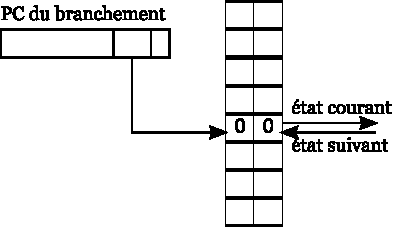
\includegraphics[scale=1]{./figures/2-bits.pdf}
      \caption{Prédicteur bimodal}
      \label{2-bit}
\end{figure}

\begin{figure}[htb]
	\center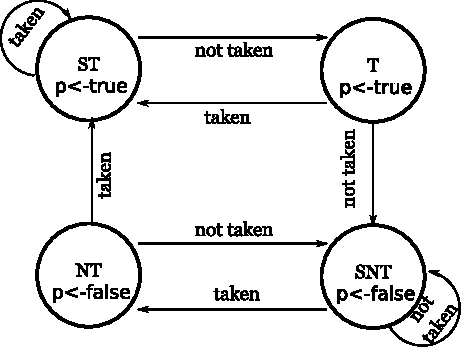
\includegraphics[scale=0.7]{./figures/2bg1.pdf}
	\caption{Automate d'un compteur 2-bit bimodal}
	\label{bimod}
\end{figure}

\section{Travail demandé} 
On implantera différents prédicteurs en prenant soin de paramétrer les tailles afin de pouvoir lancer facilement plusieurs exécutions (\emph{cf.} l'exemple fourni) et ainsi pouvoir tracer des courbes et voir les asymptotes. \textbf{Important :} Les figures montrent souvent des prédicteurs de petites tailles, mais vous êtes invités à considérer des prédicteurs commençant au moins à 128 entrées (log2(128) = 7). Lors de l'évaluation de chaque prédicteur, vous êtes invités à analyser son comportement en isolation (e.g.,~un prédicteur de plus grande taille est-il toujours meilleur ?) mais aussi à le comparer aux autres types de prédicteurs (e.g.,~deux prédicteurs aux performances égales mais l'un requiert beaucoup plus d'entrées que l'autre).

\subsection{Prédicteurs simples}

On commencera par les prédicteurs relativement simples vus en cours~:




\begin{enumerate}

%   L'historique global des branchements est un registre à décalage à gauche dans lequel on injecte sur le poids faible la décision prise ($H=3$ dans la figure~\ref{global-simple}).

%\item un prédicteur \emph{gshare} qui est un prédicteur global pour lequel l'index définissant l'entrée dans la table de taille $2^n$ est calculé comme le ou-exclusif d'un registre d'historique avec le pc du branchement, comme illustré sur la figure~\ref{gshare};
%      \begin{figure}[hbt]\center\leavevmode
%      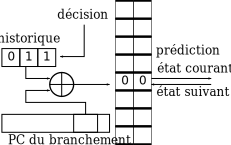
\includegraphics[scale=.9]{gshare}
%      \caption{Prédicteur \emph{gshare}}
%      \label{gshare}
%      \end{figure}
%      Si $H>n$, alors on prendra les $n$ bits de poids fort de $H$ pour faire le ou-exclusif;

\item un prédicteur \textit{gshare} qui utilise un historique global sur $H$ bits qui est combiné à l'adresse du branchement à prédire via un XOR, comme illustré sur la Figure~\ref{correlated}. 
      \begin{figure}[hbt]\center\leavevmode
      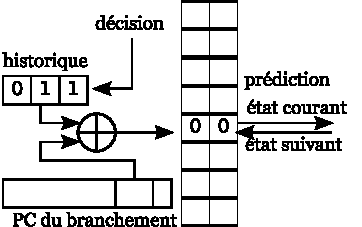
\includegraphics[scale=.9]{./figures/gshare.pdf}
      \caption{\label{correlated}Prédicteur gshare}
      \end{figure}

\item un prédicteur local qui utilise une table d'historiques sur $H$ bits (la \textit{Pattern History Table}) indexée par les poids faibles de l'adresse du branchement.  En utilisant l'entrée d'historique, on indice une BHT bimodale avec compteurs 2-bit de taille $2^H$, comme illustré sur la figure~\ref{local};
      \begin{figure}[hbt]\center\leavevmode
      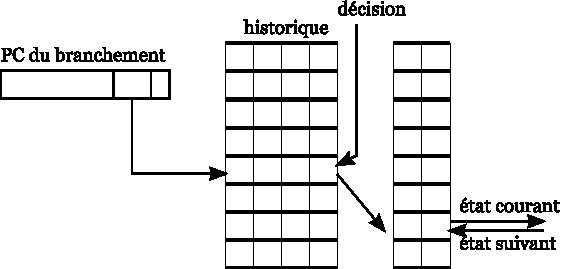
\includegraphics[scale=.9]{local}
      \caption{Prédicteur local}
      \label{local}
      \end{figure}

\item une combinaison de deux prédicteurs et le métaprédicteur associé. On va ici combiner un prédicteur global \textit{gshare} avec un historique de $H_g=10$ (soit 1024 entrées), et un prédicteur \textit{2-level} local comme celui de la précédente question, avec $H_l=10$ par entrée de la PHT (soit 1024 entrées pour la BHT, 1024 entrées pour la PHT).
La BHT indexée est un simple prédicteur bimodal.

Le choix du prédicteur à utiliser se fait grâce au métaprédicteur qui, comme les BHT des "vrais" prédicteurs, contient 1024 entrées de compteurs 2 bits. On accède au compteur en utilisant l'adresse du branchement à prédire, et ce compteur nous dit simplement quel prédicteur du prédicteur global ou du prédicteur local va effectuer la prédiction. Le compteur est incrémenté lorsque le prédicteur qui a prédit est correct et l'autre prédicteur a fait le mauvais choix, et est décrémenté dans le cas opposé (\emph{cf.} la machine d'état de la figure~\ref{mixte-graphe}). Il n'est pas nécessaire de rendre le prédicteur paramétrable. \textit{Ici, on ajoutera des statistiques afin de compter les bonnes et mauvaises prédictions de chaque prédicteur respectif, ainsi que le nombre de prédictions effectivement utilisées (i.e.,~sélectionnées par le métaprédicteur) de chaque prédicteur}.



\begin{figure}[hbt]\center\leavevmode
      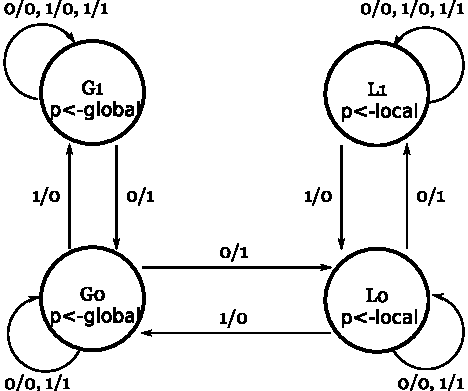
\includegraphics[scale=0.7]{./figures/mixte-graphe.pdf}
      \caption{Machine à états du choix du prédicteur.
      Légende~: $global/local$, $0$ décision incorrecte, $1$ décision correcte}
      \label{mixte-graphe}
      \end{figure}
\end{enumerate}


\subsection{Perceptron}

On se propose ensuite d'implémenter un prédicteur moderne tel que le prédicteur neural à base de perceptrons de Jiménez et Lin\footnote{\href{https://www.cs.cmu.edu/afs/cs/academic/class/15740-f18/www/papers/hpca01-jiminez-perceptron.pdf}{Lien vers "Dynamic Branch Prediction with Perceptrons".}}, et en comparer la performance avec les prédicteurs de la première partie. \\

Ce prédicteur utilise la version la plus simple des réseaux de neurones appelés perceptrons, puisqu'il n'utilise qu'une seule couche de neurones. Un perceptron "apprend" une fonction booléenne à $n$ entrée, et dans le cas du prédicteur de Jiménez et Lin, ces $n$ entrées correspondent aux bits de l'historique global de branchement (le même que dans \textit{gshare}). La sortie étant la direction prédite pour le branchement. Le modèle mathématique utilisé pour un tel perceptron est donné dans la Figure \ref{1perceptron}. Dans la Figure, $y$ dénote un vecteur de poids $w\_i$ (entiers signés), et le calcul effectué par le perceptron est le produit scalaire des entrées avec le vecteur de poids. Dans ce modèle, on ajoute une entrée $x\_0$ valant toujours 1 pour biaiser le résultat. Dans ce modèle, la valeur des entrées $x_i$ est soit $-1$ (branchement non pris) soit $1$ (branchement pris). Un résultat de la somme négatif est interprété comme la prédiction "non-pris", et un résultat positif est interprété comme la prédiction "pris".

\begin{figure}[hbt]\center\leavevmode
	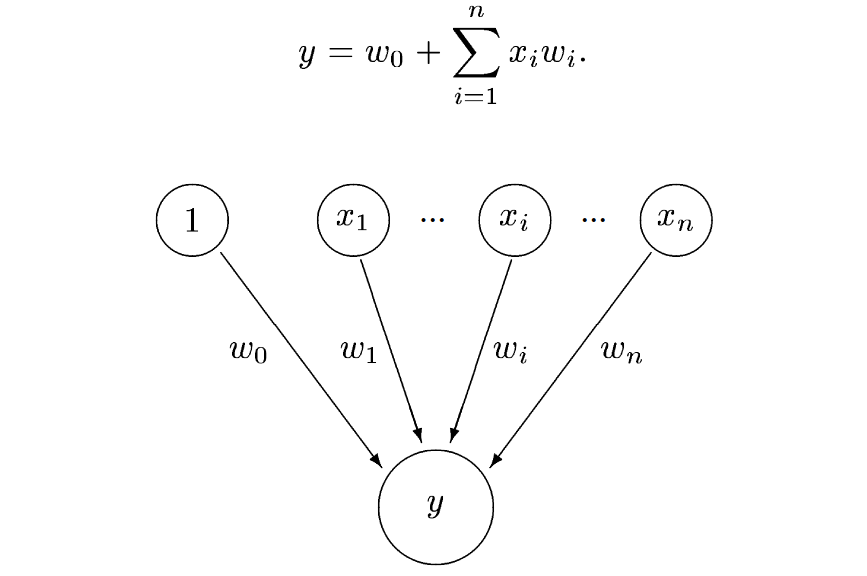
\includegraphics[width=0.5\linewidth]{1perceptron}
	\caption{Perceptron}
	\label{1perceptron}
\end{figure}

      \begin{figure}[hbt]\center\leavevmode
	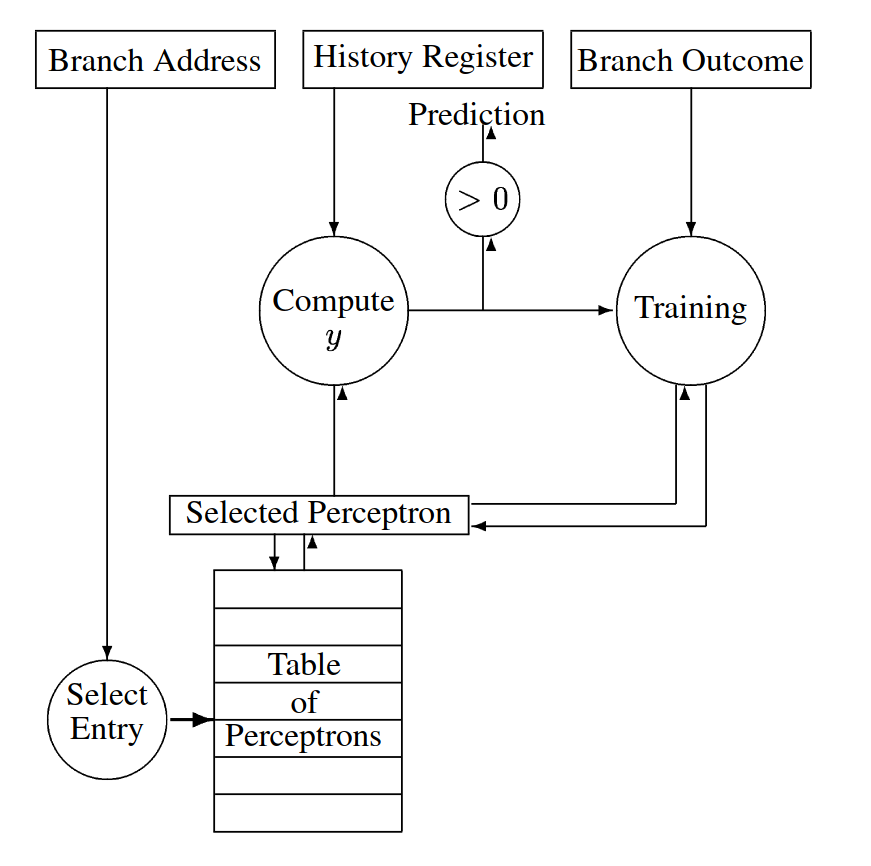
\includegraphics[width=0.5\linewidth]{perceptron}
	\caption{Prédicteur neural à base de perceptrons}
	\label{perceptron}
\end{figure}

Le diagramme du prédicteur, emprunté au papier de Jiménez et Lin est donné en Figure \ref{perceptron}. Afin de prédire la direction d'un branchement conditionnel, un tableau de perceptrons est indexé via l'adresse du branchement à prédire. Chaque entrée de la structure modélise un perceptron tel que décrit dans le paragraphe précédent. Pour générer la prédiction, le prédicteur va donc effectuer le produit scalaire du vecteur de poids (le perceptron) et le contenu du GHR (sans oublier le biais!) \\

Une fois la direction réelle du branchement obtenu, il convient de mettre à jour le prédicteurs. Ici, cela revient à mettre à jours les poids du vecteur de poids du perceptron utilisé pour prédire. On utilisera l'algorithme suivant~:

\begin{equation*}
\text{Soit~} t = -1 \text{~si le branchement est non-pris, 1 sinon}
\end{equation*}

\vspace*{-20px}

\begin{equation*}
\text{Soit~} \theta \text{~le \textit{seuil}, un paramètre de l'algorithme de mise à jour}
\end{equation*}

\vspace*{-20px}

\begin{equation*}
\text{Soit~} y_{out}=\left\{
\begin{array}{@{}ll@{}}
1, & \text{si~} y > \theta \\
0, & \text{si~} -\theta \leq y \leq \theta \\
-1, & \text{si~} y < \theta
\end{array}\right.
\end{equation*} 

\begin{equation*}
\begin{array}{@{}ll@{}}
\text{si~}y_{out} \neq t \text{~alors:} \\
  \text{~~~~pour $i := 0$ à $n$, faire}: \\
    \text{~~~~~~~~} w_i := w_i + t.x_i \\
  \text{~~~~finpour} \\
\text{finsi}
\end{array}
\end{equation*}

L'article de Jiménez et Lin suggère d'utiliser un historique global de branchement entre 12 et 62 bits suivant le budget matériel (en KB), des poids de 7 à 9 bits, mais ne donne pas de valeur pour $\theta$.

Dans le cadre de ce TP, on se limitera à un historique global de même taille que pour gshare, avec un nombre de perceptrons similaires, et on s'attachera à comparer la performance des deux prédicteurs, car il s'agit de deux prédicteurs à corrélation globale. Avant d'effectuer cette analyse, il conviendra cependant de trouver un $\theta$ donnant de bonnes performances, et éventuellement de donner une intuition sur pourquoi. 



\subsection{Aller plus loin}

L'idée de cette dernière partie est de choisir un des prédicteurs implémentés dans les parties précédentes et de chercher à minimiser les MPKI par tous les moyens possibles : taille des tables, fonction de hachage, associativité, combinaisons de prédicteurs, type d'historique (dans la mesure de ce que permet le simulateur), tout est permis. Ici, on vous encourage à analyser les traces, par exemple en construisant des statistiques sur chaque branchement dans la fonction \textit{UpdatePredictor()}, afin de tenter de déterminer pourquoi un branchement est mal prédit alors qu'il a l'air régulier ou corrélé à un voisin. Dans votre rapport, il conviendra d'expliquer les techniques utilisées et vos analyses quand à ce qui fonctionne le mieux.

\section{Infrastructure}

Il y a un script \verb+sle3a-doit.sh+ dans le répertoire \verb+script+ qui lance automatiquement l'exécution sur un sous-ensemble des traces pour un prédicteur donné, qu'il a fallut préalablement compiler dans le répertoire \verb+sim+.
Il y a dans le script pour le prédicteur $n$-modal 2 boucles imbriquées~: la boucle externe, indice $i$, fait varier le nombre de bits du compteur, et la boucle interne, d'indice $j$, fait varier le nombre de bits de PC à utiliser pour indexer les tables.
Vous serez amené à modifier les valeurs des bornes en fonction des prédicteurs, voir à changer un peu cette partie si vous faites des prédicteurs exotiques.

Le script \verb+sle3a-doit.sh+ produit ses résultats dans \verb+../results/xxx+, ou \verb+xxx+ est un répertoire dont le nom peut-être choisi à l'envie.
Il les analyse ensuite et génère des programmes \texttt{python} qui servent à tracer des courbes (avec \texttt{matplotlib}). Ces courbes sont crées dans le répertoire où on appelle \verb+sle3a-doit.sh+ et ce sont ces courbes que l'on vous demande d'analyser. \\

On donne sur la figure~\ref{results} le type de résultat attendu pour le prédicteur n-bit.

      \begin{figure}[h]
      \centering
      \subfigure[1 bit par compteur]{
      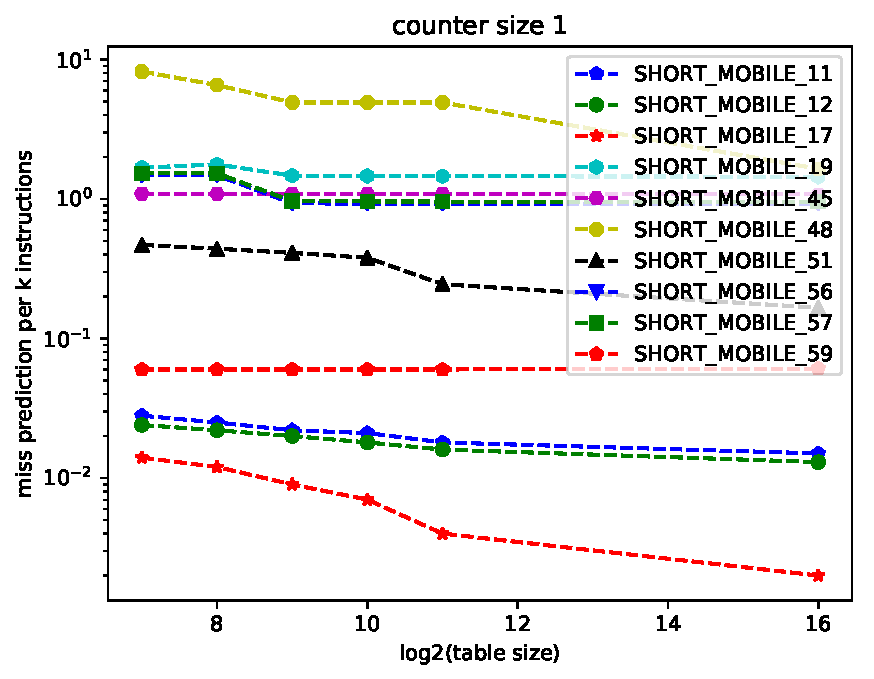
\includegraphics[scale=.48]{figures/graph_1.pdf}
      \label{plot1}
      }
      \subfigure[2 bits par compteur]{
      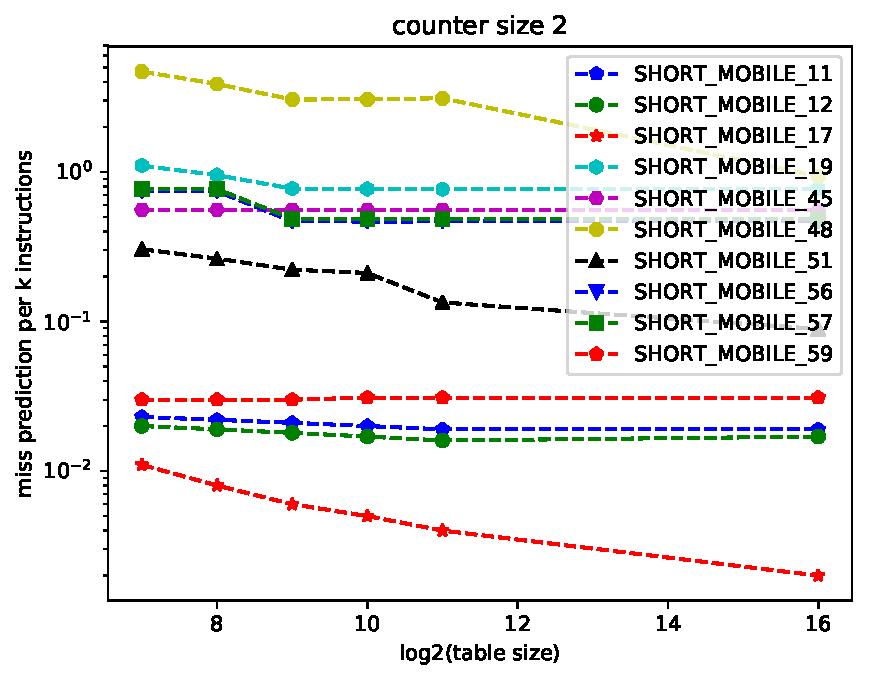
\includegraphics[scale=.48]{figures/graph_2.pdf}
      \label{plot2}
      }
      \subfigure[3 bits par compteur]{
      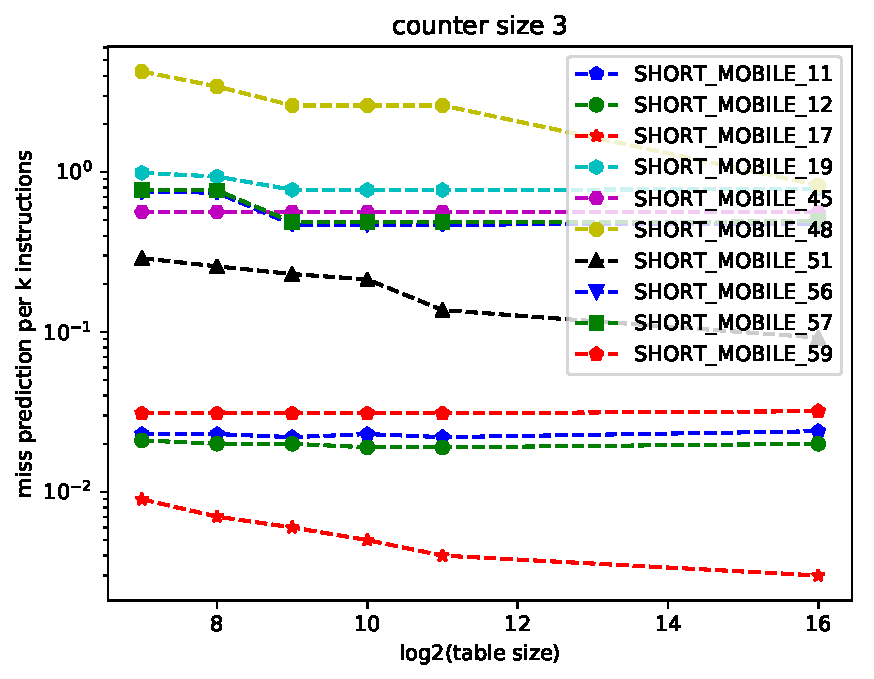
\includegraphics[scale=.48]{./figures/graph_3.pdf}
      \label{plot3}
      }
      \subfigure[4 bits par compteur]{
      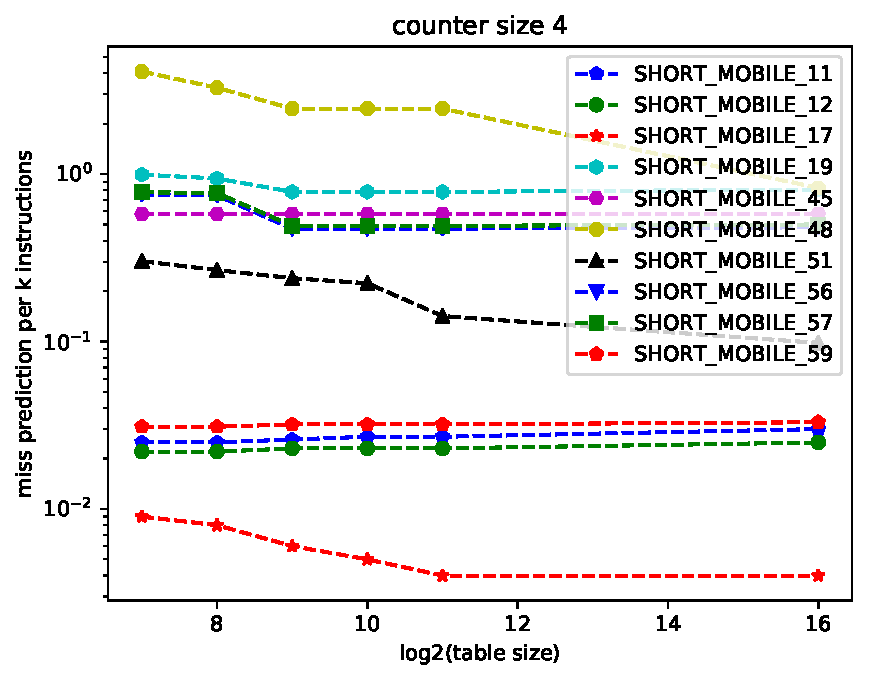
\includegraphics[scale=.48]{./figures/graph_4.pdf}
      \label{plot4}
      }
      \subfigure[5 bits par compteur]{
      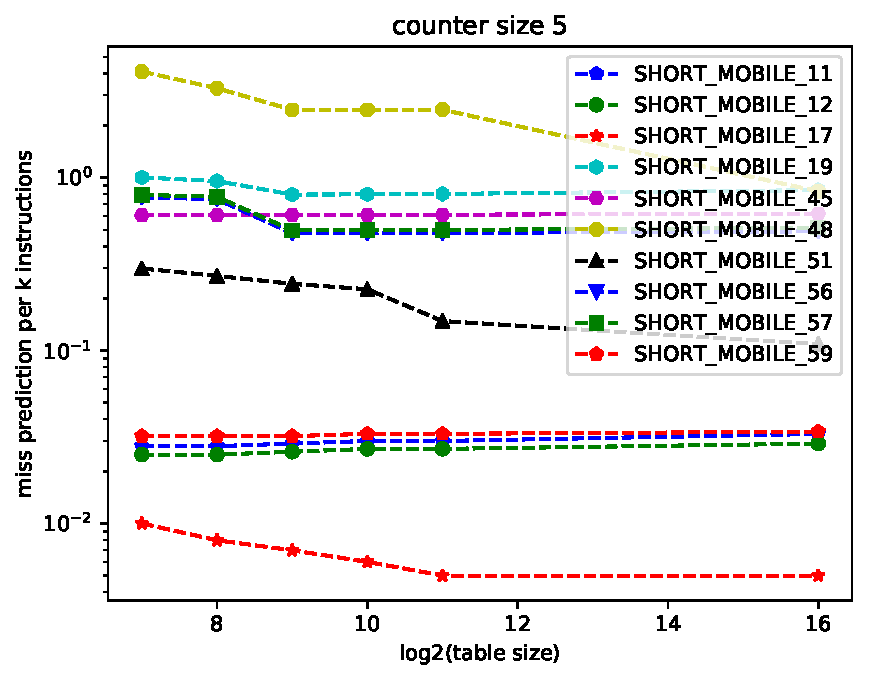
\includegraphics[scale=.48]{./figures/graph_5.pdf}
      \label{plot3}
      }
      \subfigure[6 bits par compteur]{
      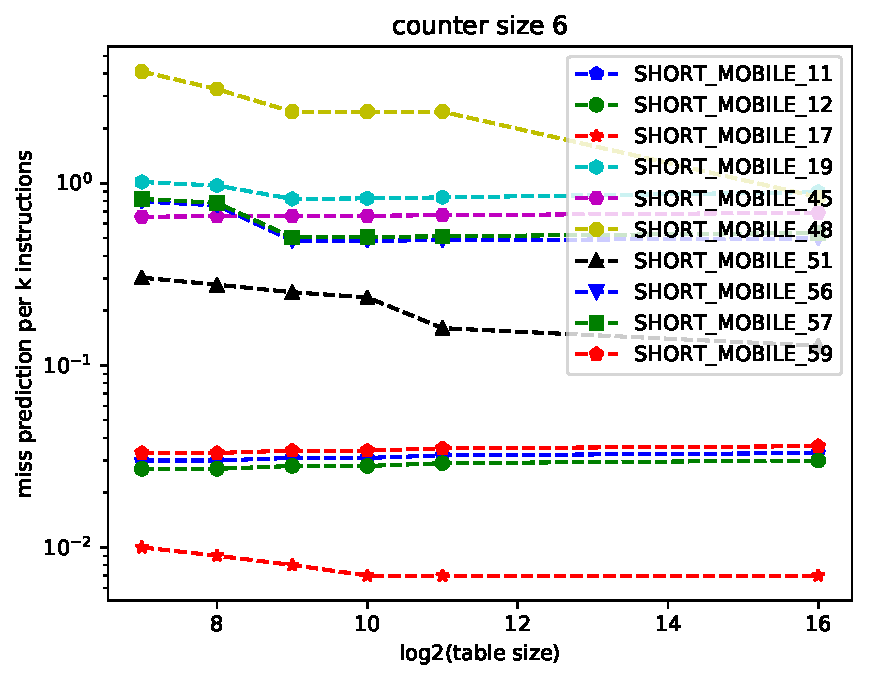
\includegraphics[scale=.48]{./figures/graph_6.pdf}
      \label{plot4}
      }
      \caption{\label{results}Les courbes de MPKI pour le prédicteur bimodal simple, en fonction du nombre de bits par compteur et du nombre d'entrées.}
      \end{figure}


\end{document}
